\documentclass[conference]{IEEEtran} % puedes cambiar a article si prefieres

\usepackage[utf8]{inputenc}
\usepackage{graphicx}
\usepackage{amsmath}
\usepackage{hyperref}
\usepackage{cite}
\usepackage{float}

\title{Validación a gran escala y Análisis de la Capacidad de Rechazo en la Memoria Asociativa Entrópica}

\author{
    Angel Fernando Bórquez Guerrero \\
    Rafael Morales Gamboa \\
}

\begin{document}

\maketitle

% -------------------- Abstract --------------------
\begin{abstract}
La Memoria Asociativa Entrópica (EAM), propuesta por Pineda y Morales (2023), constituye un modelo computacional inspirado en la cognición humana que combina propiedades de reconocimiento probabilístico con una arquitectura eficiente de almacenamiento y recuperación de patrones. En estudios previos, la EAM fue evaluada utilizando el conjunto de datos Fashion MNIST, obteniendo resultados positivos en la clasificación y reconstrucción de imágenes, aunque con la limitación de operar en un dominio reducido de solo diez clases. 

En este trabajo se presentan dos contribuciones principales orientadas a superar estas limitaciones. En primer lugar, se evalúa la escalabilidad del modelo al migrar a un conjunto de datos sustancialmente mayor: \emph{Quick, Draw!} de Google, con más de 300 clases y cientos de miles de ejemplos por categoría. En segundo lugar, se diseña un experimento de rechazo que permite verificar si la memoria es capaz de identificar y no reconocer aquellas clases que no fueron almacenadas explícitamente. Para ello, la memoria se entrena con solo la mitad de las clases y se evalúa sobre el conjunto completo. 

Los resultados obtenidos confirman que la EAM puede adaptarse a escenarios de mayor complejidad y sugieren que puede ofrecer un mecanismo efectivo de rechazo frente a estímulos inéditos, aportando evidencia de su potencial como modelo explicable y robusto dentro del campo de la inteligencia artificial.
\end{abstract}



% -------------------- Keywords --------------------
\begin{IEEEkeywords}
Memoria Asociativa Entrópica, Quick Draw, Fashion MNIST, escalabilidad, open-set recognition
\end{IEEEkeywords}



% -------------------- Introducción --------------------
\section{Introducción}

\noindent El desarrollo de modelos de memoria inspirados en la cognición humana constituye un área de investigación en creciente expansión dentro de la inteligencia artificial (IA) [REFS]. Estos enfoques buscan reproducir de manera computacional la capacidad de los sistemas biológicos para almacenar, asociar y recuperar información a partir de experiencias previas. En este contexto, la \textit{Memoria Asociativa Entrópica} (EAM, por sus siglas en inglés) propuesta por Pineda y Morales \cite{pinedaImageryEntropicAssociative2023} representa un avance teórico significativo al ofrecer una arquitectura declarativa, distribuida y eficiente, capaz de realizar reconocimiento probabilístico y recuperación flexible de patrones.

Los estudios iniciales con la EAM se enfocaron en conjuntos de datos clásicos y relativamente pequeños como \textit{Fashion MNIST} \cite{zalandoresearchFashionMNIST2022}, un conjunto con 70,000 imágenes distribuidas en 10 clases de objetos. En este dominio, el modelo demostró ser capaz de almacenar representaciones latentes generadas por un autoencoder convolucional y de recuperar dichas representaciones incluso en presencia de ruido o información incompleta. Estos resultados validaron la eficacia del modelo en tareas de reconocimiento cerrado, donde todas las clases de prueba (no así las instancias) habían sido registradas en memoria.

Sin embargo, el marco experimental original presentaba tres limitaciones principales. En primer lugar, la evaluación se realizó en un dominio pequeño y limitado, lo cual restringía el análisis de escalabilidad del modelo. En segundo lugar, no se había probado de manera explícita la capacidad de la memoria para rechazar instancias de clases no registradas, un aspecto crítico en problemas de \emph{open-set recognition} \cite{scheirerOpenSetRecognition2013}.

El presente trabajo busca superar estas limitaciones a través de dos líneas de investigación: (1) evaluar la escalabilidad de la EAM utilizando el conjunto de datos \textit{Quick, Draw!} \cite{googlecreativelabQuickDrawData2025}, con más de 300 clases y cientos de miles de ejemplos por categoría; (2) diseñar un experimento de rechazo que permita observar el desempeño de la memoria en no reconocer clases no almacenadas.

De esta manera, el artículo contribuye a ampliar la comprensión del comportamiento de la Memoria Asociativa Entrópica en escenarios más complejos, aportando evidencia empírica sobre su robustez, su capacidad de generalización y su potencial como paradigma alternativo dentro de la inteligencia artificial explicable.



% -------------------- Antecedentes --------------------
\section{Antecedentes}

\noindent La \textit{Memoria Asociativa Entrópica} (EAM, por sus siglas en inglés), propuesta por Pineda y Morales \cite{pinedaImageryEntropicAssociative2023}, surge como un modelo computacional inspirado en la cognición humana cuyo propósito es almacenar y recuperar patrones de manera probabilística y distribuida. A diferencia de los sistemas de memoria convencionales, la EAM opera sobre un único registro asociativo (\textit{Associative Memory Register}) que concentra las asociaciones de todos los patrones aprendidos en una representación matricial. Este enfoque permite un comportamiento flexible en el reconocimiento y la recuperación, y abre la puerta al estudio de fenómenos emergentes como la generalización y la generación de imágenes sintéticas.

El modelo se fundamenta en tres operaciones principales: 
\begin{itemize}
    \item \textbf{$\lambda$-register}: registra un patrón en la memoria reforzando las asociaciones entre sus características.
    \item \textbf{$\eta$-recognition}: determina si un estímulo de entrada es reconocido por la memoria, utilizando un criterio de tolerancia a errores y umbrales de confianza.
    \item \textbf{$\beta$-retrieval}: recupera un patrón completo a partir de una pista, que puede ser parcial o con ruido, utilizando distribuciones probabilísticas sobre las asociaciones almacenadas.
\end{itemize}
%
En experimentos previos, la EAM fue evaluada con el conjunto de datos \textit{Fashion MNIST} \cite{zalandoresearchFashionMNIST2022}, compuesto por 70,000 imágenes distribuidas en 10 clases. En este escenario, la memoria fue alimentada con representaciones latentes producidas por un autoencoder convolucional, y demostró capacidad tanto para reconocer como para reconstruir patrones aún en condiciones de ruido o información incompleta. Asimismo, se exploraron fenómenos emergentes como la generación de secuencias de recuerdos (\textit{association chains}), mostrando la capacidad del sistema para transitar entre representaciones almacenadas. Posteriormente, se realizó un primer estudio utilizando el conjunto de datos \emph{Quick, Draw!} de Google, con pequeñas variaciones en el número de clases (entre 10 y 13), con resultados aceptables \cite{gonzalez2024clasificador}.

A pesar de estos resultados prometedores, el marco experimental original presentaba limitaciones relevantes: 
(1) la evaluación se restringió a un conjunto reducido de 10 clases, lo que dificultaba analizar la escalabilidad del modelo en contextos más complejos; 
(2) no se realizaron pruebas sistemáticas sobre la capacidad de la memoria para rechazar patrones de clases no vistas, un aspecto fundamental en el reconocimiento de conjuntos abiertos; y 
(3) el diseño experimental estaba acoplado al número fijo de clases configuradas en las redes neuronales, limitando la flexibilidad para explorar diferentes configuraciones de carga de memoria.

Estas limitaciones motivan el presente trabajo, cuyo objetivo es validar la EAM en un entorno más desafiante mediante la migración al conjunto de datos \textit{Quick, Draw!} \cite{googlecreativelabQuickDrawData2025} y el diseño de un experimento específico para analizar su capacidad de rechazo frente a clases inéditas.



% -------------------- Metodología --------------------
\section{Metodología}

\noindent Con el objetivo de extender la validación del modelo de Memoria Asociativa Entrópica (EAM) y analizar su comportamiento en escenarios más complejos, se diseñó una metodología experimental dividida en tres fases principales. Estas fases permitieron migrar a un nuevo dominio de datos, evaluar el mecanismo de rechazo explícito y dotar al sistema de mayor flexibilidad para futuros experimentos.

\subsection{Migración del conjunto de datos y validación a gran escala}
\noindent El primer paso consistió en reemplazar el conjunto de datos \textit{Fashion MNIST} por \textit{Quick. Draw!} \cite{googlecreativelabQuickDrawData2025}, con más de 300 clases y cientos de miles de ejemplos por categoría. Este proceso requirió:
\begin{itemize}
    \item \textbf{Adaptación del módulo de datos:} Se modificó el script \texttt{dataset.py} para cargar, procesar y balancear dinámicamente clases de \emph{Quick, Draw!}. La lógica se ajustó para manejar un número variable de categorías y garantizar un número equitativo de muestras por clase.
    \item \textbf{Reentrenamiento de las redes neuronales:} Se ajustó el sistema perceptivo, consistente en un autocodificador y un clasificador (definido en \texttt{neural\_net.py}), con base en el trabajo realizado para \cite{moralesMissingCueProblem2025} y se entrenó desde cero el sistema perceptivo  utilizando \emph{Quick, Draw!} como nueva fuente de datos. Este paso generó representaciones latentes (\textit{features}) adecuadas para la memoria.
    \item \textbf{Validación del \emph{pipeline}:} Se ejecutó el flujo completo (entrenamiento del autoencodificador-clasificador, generación de características, almacenamiento en memoria y evaluación de reconocimiento) para verificar la compatibilidad del modelo con el nuevo dominio.
\end{itemize}

\subsection{Diseño e implementación del experimento de rechazo}
\noindent Para analizar la capacidad del sistema de rechazar patrones de clases no vistas, se implementó un segundo experimento con la siguiente lógica:
\begin{itemize}
    \item \textbf{Extensión de la interfaz de comandos:} Se añadió un nuevo argumento en el programa principal \texttt{eam.py} (\texttt{-e 2}) para invocar este modo experimental.
    \item \textbf{Registro parcial en memoria:} Aunque el clasificador fue entrenado con todas las clases seleccionadas, en la EAM se registró únicamente la mitad de ellas.
    \item \textbf{Evaluación con conjunto completo:} En la fase de prueba, el sistema se expuso a todas las clases, incluyendo las no registradas, lo que permitió evaluar explícitamente su respuesta de rechazo.
    \item \textbf{Métrica de aceptación y rechazo:} Se empleó el índice \texttt{no\_response} como medida cuantitativa para evaluar la capacidad del sistema de no asociar patrones pertenecientes a clases no vistas.
\end{itemize}

\subsection{Refactorización para la flexibilidad experimental}
\noindent Con el fin de transformar el sistema en una plataforma experimental más versátil, se llevaron a cabo modificaciones adicionales:
\begin{itemize}
    \item \textbf{Parametrización del número de clases:} El programa \texttt{eam.py} fue modificado para aceptar el número de clases como argumento de ejecución (\texttt{<classes>}), en lugar de estar fijado en el código.
    \item \textbf{Propagación de parámetros:} Este valor fue transmitido al módulo de datos, lo que permitió preparar dinámicamente sólo el subconjunto de clases requerido.
    \item \textbf{Carga dinámica:} El sistema quedó habilitado para realizar experimentos con diferentes cantidades de clases (2, 4, 8, 16, 24 o 32), adaptándose a escenarios controlados de diversa complejidad.
\end{itemize}
%
En conjunto, estas tres fases metodológicas permitieron escalar el modelo hacia un dominio sustancialmente mayor, analizar su capacidad de rechazo ante estímulos inéditos y habilitar una infraestructura más flexible para futuras pruebas experimentales.



% -------------------- Resultados --------------------

\section{Resultados}

\subsection{Resultados cuantitativos por Número de Clases}
En esta subsección se muestran las gráficas que resumen el comportamiento promedio y la precisión de la memoria al variar el número de clases (2, 4, 8, 16, 24 y 32). 

% -- 2 Clases
\begin{figure}[H]
    \centering
    \includegraphics[width=0.45\textwidth]{Graficas/runs_02/graph_behaviours_MEAN-english.pdf}
    \caption{Comportamiento promedio de la memoria con 2 clases.}
    \label{fig:behaviours_2}
\end{figure}

\begin{figure}[H]
    \centering
    \includegraphics[width=0.45\textwidth]{Graficas/runs_02/graph_prse_MEAN-english.pdf}
    \caption{Precisión global del sistema con 2 clases.}
    \label{fig:precision_2}
\end{figure}

% -- 4 Clases
\begin{figure}[H]
    \centering
    \includegraphics[width=0.45\textwidth]{Graficas/runs_04/graph_behaviours_MEAN-english.pdf}
    \caption{Comportamiento promedio de la memoria con 4 clases.}
    \label{fig:behaviours_4}
\end{figure}

\begin{figure}[H]
    \centering
    \includegraphics[width=0.45\textwidth]{Graficas/runs_04/graph_prse_MEAN-english.pdf}
    \caption{Precisión global del sistema con 4 clases.}
    \label{fig:precision_4}
\end{figure}

% -- 8 Clases
\begin{figure}[H]
    \centering
    \includegraphics[width=0.45\textwidth]{Graficas/runs_08/graph_behaviours_MEAN-english.pdf}
    \caption{Comportamiento promedio de la memoria con 8 clases.}
    \label{fig:behaviours_8}
\end{figure}

\begin{figure}[H]
    \centering
    \includegraphics[width=0.45\textwidth]{Graficas/runs_08/graph_prse_MEAN-english.pdf}
    \caption{Precisión global del sistema con 8 clases.}
    \label{fig:precision_8}
\end{figure}

% -- 16 Clases
\begin{figure}[H]
    \centering
    \includegraphics[width=0.45\textwidth]{Graficas/runs_16/graph_behaviours_MEAN-english.pdf}
    \caption{Comportamiento promedio de la memoria con 16 clases.}
    \label{fig:behaviours_16}
\end{figure}

\begin{figure}[H]
    \centering
    \includegraphics[width=0.45\textwidth]{Graficas/runs_16/graph_prse_MEAN-english.pdf}
    \caption{Precisión global del sistema con 16 clases.}
    \label{fig:precision_16}
\end{figure}

% -- 24 Clases
\begin{figure}[H]
    \centering
    \includegraphics[width=0.45\textwidth]{Graficas/runs_24/graph_behaviours_MEAN-english.pdf}
    \caption{Comportamiento promedio de la memoria con 24 clases.}
    \label{fig:behaviours_24}
\end{figure}

\begin{figure}[H]
    \centering
    \includegraphics[width=0.45\textwidth]{Graficas/runs_24/graph_prse_MEAN-english.pdf}
    \caption{Precisión global del sistema con 24 clases.}
    \label{fig:precision_24}
\end{figure}

% -- 32 Clases
\begin{figure}[H]
    \centering
    \includegraphics[width=0.45\textwidth]{Graficas/runs_32/graph_behaviours_MEAN-english.pdf}
    \caption{Comportamiento promedio de la memoria con 32 clases.}
    \label{fig:behaviours_32}
\end{figure}

\begin{figure}[H]
    \centering
    \includegraphics[width=0.45\textwidth]{Graficas/runs_32/graph_prse_MEAN-english.pdf}
    \caption{Precisión global del sistema con 32 clases.}
    \label{fig:precision_32}
\end{figure}


% --------------------


\subsection{Resultados del Experimento 1 (Todas las clases registradas)}
En este experimento, la memoria almacenó todas las clases disponibles. Se presentan las gráficas de recall correspondientes a diferentes configuraciones de tamaño de memoria (\texttt{sze}).

% -- 2 Clases
\begin{figure}[H]
    \centering
    \includegraphics[width=0.45\textwidth]{Graficas/runs_02/recall-exp_001-sze_004-graph_prse_MEAN-english.pdf}
    \caption{Recall del experimento 1 con 2 clases y tamaño de memoria \texttt{sze=004}.}
    \label{fig:recall_exp1_2_004}
\end{figure}

\begin{figure}[H]
    \centering
    \includegraphics[width=0.45\textwidth]{Graficas/runs_02/recall-exp_001-sze_008-graph_prse_MEAN-english.pdf}
    \caption{Recall del experimento 1 con 2 clases y tamaño de memoria \texttt{sze=008}.}
    \label{fig:recall_exp1_2_008}
\end{figure}

\begin{figure}[H]
    \centering
    \includegraphics[width=0.45\textwidth]{Graficas/runs_02/recall-exp_001-sze_032-graph_prse_MEAN-english.pdf}
    \caption{Recall del experimento 1 con 2 clases y tamaño de memoria \texttt{sze=032}.}
    \label{fig:recall_exp1_2_032}
\end{figure}


% -- 4 Clases
\begin{figure}[H]
    \centering
    \includegraphics[width=0.45\textwidth]{Graficas/runs_04/recall-exp_001-sze_002-graph_prse_MEAN-english.pdf}
    \caption{Recall del experimento 1 con 4 clases y tamaño de memoria \texttt{sze=002}.}
    \label{fig:recall_exp1_4_002}
\end{figure}

\begin{figure}[H]
    \centering
    \includegraphics[width=0.45\textwidth]{Graficas/runs_04/recall-exp_001-sze_004-graph_prse_MEAN-english.pdf}
    \caption{Recall del experimento 1 con 4 clases y tamaño de memoria \texttt{sze=004}.}
    \label{fig:recall_exp1_4_004}
\end{figure}

\begin{figure}[H]
    \centering
    \includegraphics[width=0.45\textwidth]{Graficas/runs_04/recall-exp_001-sze_016-graph_prse_MEAN-english.pdf}
    \caption{Recall del experimento 1 con 4 clases y tamaño de memoria \texttt{sze=016}.}
    \label{fig:recall_exp1_4_016}
\end{figure}


% -- 8 Clases
\begin{figure}[H]
    \centering
    \includegraphics[width=0.45\textwidth]{Graficas/runs_08/recall-exp_001-sze_004-graph_prse_MEAN-english.pdf}
    \caption{Recall del experimento 1 con 8 clases y tamaño de memoria \texttt{sze=004}.}
    \label{fig:recall_exp1_8_004}
\end{figure}

\begin{figure}[H]
    \centering
    \includegraphics[width=0.45\textwidth]{Graficas/runs_08/recall-exp_001-sze_008-graph_prse_MEAN-english.pdf}
    \caption{Recall del experimento 1 con 8 clases y tamaño de memoria \texttt{sze=008}.}
    \label{fig:recall_exp1_8_008}
\end{figure}

\begin{figure}[H]
    \centering
    \includegraphics[width=0.45\textwidth]{Graficas/runs_08/recall-exp_001-sze_016-graph_prse_MEAN-english.pdf}
    \caption{Recall del experimento 1 con 8 clases y tamaño de memoria \texttt{sze=016}.}
    \label{fig:recall_exp1_8_016}
\end{figure}


% -- 16 Clases
\begin{figure}[H]
    \centering
    \includegraphics[width=0.45\textwidth]{Graficas/runs_16/recall-exp_001-sze_004-graph_prse_MEAN-english.pdf}
    \caption{Recall del experimento 1 con 16 clases y tamaño de memoria \texttt{sze=004}.}
    \label{fig:recall_exp1_16_004}
\end{figure}

\begin{figure}[H]
    \centering
    \includegraphics[width=0.45\textwidth]{Graficas/runs_16/recall-exp_001-sze_008-graph_prse_MEAN-english.pdf}
    \caption{Recall del experimento 1 con 16 clases y tamaño de memoria \texttt{sze=008}.}
    \label{fig:recall_exp1_16_008}
\end{figure}

\begin{figure}[H]
    \centering
    \includegraphics[width=0.45\textwidth]{Graficas/runs_16/recall-exp_001-sze_016-graph_prse_MEAN-english.pdf}
    \caption{Recall del experimento 1 con 16 clases y tamaño de memoria \texttt{sze=016}.}
    \label{fig:recall_exp1_16_016}
\end{figure}


% -- 24 Clases
\begin{figure}[H]
    \centering
    \includegraphics[width=0.45\textwidth]{Graficas/runs_24/recall-exp_001-sze_032-graph_prse_MEAN-english.pdf}
    \caption{Recall del experimento 1 con 24 clases y tamaño de memoria \texttt{sze=032}.}
    \label{fig:recall_exp1_24_032}
\end{figure}

\begin{figure}[H]
    \centering
    \includegraphics[width=0.45\textwidth]{Graficas/runs_24/recall-exp_001-sze_064-graph_prse_MEAN-english.pdf}
    \caption{Recall del experimento 1 con 24 clases y tamaño de memoria \texttt{sze=064}.}
    \label{fig:recall_exp1_24_064}
\end{figure}


% -- 32 Clases
\begin{figure}[H]
    \centering
    \includegraphics[width=0.45\textwidth]{Graficas/runs_32/recall-exp_001-sze_016-graph_prse_MEAN-english.pdf}
    \caption{Recall del experimento 1 con 32 clases y tamaño de memoria \texttt{sze=016}.}
    \label{fig:recall_exp1_32_016}
\end{figure}

\begin{figure}[H]
    \centering
    \includegraphics[width=0.45\textwidth]{Graficas/runs_32/recall-exp_001-sze_032-graph_prse_MEAN-english.pdf}
    \caption{Recall del experimento 1 con 32 clases y tamaño de memoria \texttt{sze=032}.}
    \label{fig:recall_exp1_32_032}
\end{figure}


% --------------------


\subsection{Resultados del Experimento 2 (Rechazo de clases no registradas)}
En este experimento, la memoria solo registró la mitad de las clases, pero se evaluó contra el conjunto completo. Se muestran las gráficas de recall, destacando la métrica \texttt{no\_response} como indicador de rechazo.

% -- 2 Clases
\begin{figure}[H]
    \centering
    \includegraphics[width=0.45\textwidth]{Graficas/runs_02/recall-exp_002-sze_004-graph_prse_MEAN-english.pdf}
    \caption{Recall del experimento 2 con 2 clases y tamaño de memoria \texttt{sze=004}.}
    \label{fig:recall_exp2_2_004}
\end{figure}

\begin{figure}[H]
    \centering
    \includegraphics[width=0.45\textwidth]{Graficas/runs_02/recall-exp_002-sze_008-graph_prse_MEAN-english.pdf}
    \caption{Recall del experimento 2 con 2 clases y tamaño de memoria \texttt{sze=008}.}
    \label{fig:recall_exp2_2_008}
\end{figure}

\begin{figure}[H]
    \centering
    \includegraphics[width=0.45\textwidth]{Graficas/runs_02/recall-exp_002-sze_032-graph_prse_MEAN-english.pdf}
    \caption{Recall del experimento 2 con 2 clases y tamaño de memoria \texttt{sze=032}.}
    \label{fig:recall_exp2_2_032}
\end{figure}


% -- 4 Clases
\begin{figure}[H]
    \centering
    \includegraphics[width=0.45\textwidth]{Graficas/runs_04/recall-exp_002-sze_002-graph_prse_MEAN-english.pdf}
    \caption{Recall del experimento 2 con 4 clases y tamaño de memoria \texttt{sze=002}.}
    \label{fig:recall_exp2_4_002}
\end{figure}

\begin{figure}[H]
    \centering
    \includegraphics[width=0.45\textwidth]{Graficas/runs_04/recall-exp_002-sze_004-graph_prse_MEAN-english.pdf}
    \caption{Recall del experimento 2 con 4 clases y tamaño de memoria \texttt{sze=004}.}
    \label{fig:recall_exp2_4_004}
\end{figure}

\begin{figure}[H]
    \centering
    \includegraphics[width=0.45\textwidth]{Graficas/runs_04/recall-exp_002-sze_032-graph_prse_MEAN-english.pdf}
    \caption{Recall del experimento 2 con 4 clases y tamaño de memoria \texttt{sze=032}.}
    \label{fig:recall_exp2_4_032}
\end{figure}


% -- 8 Clases
\begin{figure}[H]
    \centering
    \includegraphics[width=0.45\textwidth]{Graficas/runs_08/recall-exp_002-sze_004-graph_prse_MEAN-english.pdf}
    \caption{Recall del experimento 2 con 8 clases y tamaño de memoria \texttt{sze=004}.}
    \label{fig:recall_exp2_8_004}
\end{figure}

\begin{figure}[H]
    \centering
    \includegraphics[width=0.45\textwidth]{Graficas/runs_08/recall-exp_002-sze_008-graph_prse_MEAN-english.pdf}
    \caption{Recall del experimento 2 con 8 clases y tamaño de memoria \texttt{sze=008}.}
    \label{fig:recall_exp2_8_008}
\end{figure}

\begin{figure}[H]
    \centering
    \includegraphics[width=0.45\textwidth]{Graficas/runs_08/recall-exp_002-sze_016-graph_prse_MEAN-english.pdf}
    \caption{Recall del experimento 2 con 8 clases y tamaño de memoria \texttt{sze=016}.}
    \label{fig:recall_exp2_8_016}
\end{figure}


% -- 16 Clases
\begin{figure}[H]
    \centering
    \includegraphics[width=0.45\textwidth]{Graficas/runs_16/recall-exp_002-sze_004-graph_prse_MEAN-english.pdf}
    \caption{Recall del experimento 2 con 16 clases y tamaño de memoria \texttt{sze=004}.}
    \label{fig:recall_exp2_16_004}
\end{figure}

\begin{figure}[H]
    \centering
    \includegraphics[width=0.45\textwidth]{Graficas/runs_16/recall-exp_002-sze_008-graph_prse_MEAN-english.pdf}
    \caption{Recall del experimento 2 con 16 clases y tamaño de memoria \texttt{sze=008}.}
    \label{fig:recall_exp2_16_008}
\end{figure}

\begin{figure}[H]
    \centering
    \includegraphics[width=0.45\textwidth]{Graficas/runs_16/recall-exp_002-sze_016-graph_prse_MEAN-english.pdf}
    \caption{Recall del experimento 2 con 16 clases y tamaño de memoria \texttt{sze=016}.}
    \label{fig:recall_exp2_16_016}
\end{figure}


% -- 24 Clases
\begin{figure}[H]
    \centering
    \includegraphics[width=0.45\textwidth]{Graficas/runs_24/recall-exp_002-sze_032-graph_prse_MEAN-english.pdf}
    \caption{Recall del experimento 2 con 24 clases y tamaño de memoria \texttt{sze=032}.}
    \label{fig:recall_exp2_24_032}
\end{figure}

\begin{figure}[H]
    \centering
    \includegraphics[width=0.45\textwidth]{Graficas/runs_24/recall-exp_002-sze_064-graph_prse_MEAN-english.pdf}
    \caption{Recall del experimento 2 con 24 clases y tamaño de memoria \texttt{sze=064}.}
    \label{fig:recall_exp2_24_064}
\end{figure}


% -- 32 Clases
\begin{figure}[H]
    \centering
    \includegraphics[width=0.45\textwidth]{Graficas/runs_32/recall-exp_002-sze_016-graph_prse_MEAN-english.pdf}
    \caption{Recall del experimento 2 con 32 clases y tamaño de memoria \texttt{sze=016}.}
    \label{fig:recall_exp2_32_016}
\end{figure}

\begin{figure}[H]
    \centering
    \includegraphics[width=0.45\textwidth]{Graficas/runs_32/recall-exp_002-sze_032-graph_prse_MEAN-english.pdf}
    \caption{Recall del experimento 2 con 32 clases y tamaño de memoria \texttt{sze=032}.}
    \label{fig:recall_exp2_32_032}
\end{figure}


% --------------------


\subsection{Clasificador base}
Finalmente, se incluyen las matrices de confusión generadas por el clasificador previo a la memoria para cada configuración de clases.

\begin{figure}[H]
    \centering
    \includegraphics[width=0.45\textwidth]{Graficas/runs_02/model-classifier-confrix.pdf}
    \caption{Matriz de confusión del clasificador base con 02 clases.}
    \label{fig:classifier_2}
\end{figure}

\begin{figure}[H]
    \centering
    \includegraphics[width=0.45\textwidth]{Graficas/runs_04/model-classifier-confrix.pdf}
    \caption{Matriz de confusión del clasificador base con 4 clases.}
    \label{fig:classifier_4}
\end{figure}

\begin{figure}[H]
    \centering
    \includegraphics[width=0.45\textwidth]{Graficas/runs_08/model-classifier-confrix.pdf}
    \caption{Matriz de confusión del clasificador base con 8 clases.}
    \label{fig:classifier_8}
\end{figure}

\begin{figure}[H]
    \centering
    \includegraphics[width=0.45\textwidth]{Graficas/runs_16/model-classifier-confrix.pdf}
    \caption{Matriz de confusión del clasificador base con 16 clases.}
    \label{fig:classifier_16}
\end{figure}

\begin{figure}[H]
    \centering
    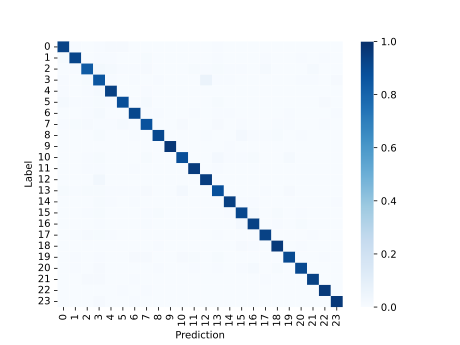
\includegraphics[width=0.45\textwidth]{Graficas/runs_24/model-classifier-confrix.pdf}
    \caption{Matriz de confusión del clasificador base con 24 clases.}
    \label{fig:classifier_24}
\end{figure}

\begin{figure}[H]
    \centering
    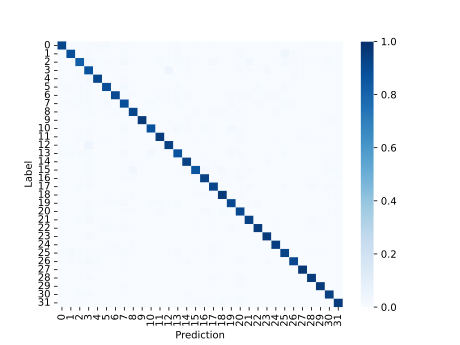
\includegraphics[width=0.45\textwidth]{Graficas/runs_32/model-classifier-confrix.pdf}
    \caption{Matriz de confusión del clasificador base con 32 clases.}
    \label{fig:classifier_32}
\end{figure}



% -------------------- Discución --------------------
\section{Discusión}

Los resultados experimentales permiten extraer varias observaciones relevantes sobre el comportamiento de la Memoria Asociativa Entrópica (EAM) en escenarios de mayor complejidad.

En primer lugar, al aumentar progresivamente el número de clases (2, 4, 8, 16, 24 y 32), se observó una tendencia general a la disminución en las métricas de precisión y recall. Este comportamiento es esperado, ya que la complejidad del dominio y la variabilidad de los patrones crece con el número de categorías. No obstante, la EAM mantuvo un desempeño estable en configuraciones de baja y media complejidad, lo que confirma su capacidad para escalar más allá del dominio reducido de Fashion MNIST.

En segundo lugar, los experimentos de rechazo (Experimento 2) evidenciaron que la memoria fue capaz de identificar patrones correspondientes a clases no registradas y responder con un índice elevado de \texttt{no\_response}. Este resultado constituye una validación empírica de la hipótesis de que la EAM puede operar en escenarios de reconocimiento abierto, diferenciando entre estímulos familiares y no familiares. Sin embargo, también se detectaron casos de falsos rechazos en clases registradas, lo que sugiere la necesidad de ajustar parámetros de umbral o explorar mecanismos complementarios de discriminación.

Finalmente, la comparación con el clasificador base resalta el papel de la memoria en el sistema completo. Mientras que el clasificador aporta representaciones latentes útiles, es la EAM la que confiere la capacidad de rechazo y recuperación probabilística, aportando un valor añadido frente a arquitecturas puramente discriminativas.

En conjunto, estos hallazgos demuestran que la EAM no solo puede adaptarse a dominios más complejos, sino que también ofrece un mecanismo efectivo para tratar con información novedosa. Al mismo tiempo, ponen de manifiesto retos futuros relacionados con la optimización de sus parámetros y la evaluación en dominios aún más grandes y heterogéneos.



% -------------------- Conclusiones --------------------
\section{Conclusiones}

Este trabajo amplió el marco experimental de la Memoria Asociativa Entrópica (EAM) para evaluar su desempeño en escenarios de mayor complejidad y analizar su capacidad de rechazo ante clases no registradas. Las principales contribuciones pueden resumirse de la siguiente manera:

\begin{itemize}
    \item \textbf{Validación a gran escala:} Se migró de un dominio reducido de diez clases en Fashion MNIST a un dominio más amplio y diverso utilizando \emph{Quick, Draw!}, con resultados que confirman la capacidad del modelo para escalar en contextos con cientos de clases y mayor variabilidad en los patrones.
    
    \item \textbf{Capacidad de rechazo:} Se diseñó e implementó un nuevo experimento que mostró empíricamente cómo la EAM es capaz de emitir una respuesta de \texttt{no\_response} frente a estímulos correspondientes a clases no vistas, validando su utilidad en problemas de reconocimiento abierto.
    
    \item \textbf{Flexibilidad experimental:} El sistema fue refactorizado para aceptar un número variable de clases y distintos tamaños de memoria, lo que habilita un entorno más versátil para la exploración de configuraciones y análisis comparativos.
\end{itemize}

Los hallazgos obtenidos demuestran que la EAM constituye un modelo explicable y robusto, capaz de combinar el almacenamiento distribuido con mecanismos probabilísticos de recuperación y rechazo. Estos resultados refuerzan su potencial como paradigma alternativo dentro de la inteligencia artificial, particularmente en tareas donde la capacidad de manejar información novedosa resulta crítica.

Como trabajo futuro, se propone extender los experimentos hacia dominios aún más grandes y heterogéneos, optimizar los parámetros de umbral asociados al rechazo, e investigar la integración de la EAM con arquitecturas de aprendizaje profundo más avanzadas para fortalecer tanto su precisión como su capacidad de generalización.



% -------------------- Referencias --------------------
\bibliographystyle{IEEEtran}
\bibliography{articulo}
\end{document}
